\chapter{Detailed Classes of Attacks and Vectors}

In this appendix, we will analyze several types of attacks: IP Spoofing, Packet Sniffing, Connection Hijacking, and Distributed Denial of Service (DDoS).

\raggedright
\begin{center}
    \section{IP Spoofing} 
\end{center}
A technique where \textbf{an attacker alters the source IP address} in a packet header to disguise their identity or impersonate another system.

\subsection*{Common uses of IP spoofing}
\begin{itemize}
    \item In \textbf{Distributed Denial of Service} (DDoS) attacks, IP spoofing is employed to generate a massive amount of traffic directed at a target, using multiple spoofed IP addresses to overwhelm the target’s resources and cause a service disruption.

    \item Another use of IP spoofing is in \textbf{Man-in-the-Middle} (MITM) attacks, where attackers impersonate trusted IP addresses to intercept or alter communications between two systems, potentially reading sensitive data or injecting malicious content.

    \item In \textbf{Session Hijacking}, attackers spoof an IP address to impersonate a legitimate device, allowing them to gain unauthorized access to an active session.

    \item In \textbf{Reflection and Amplification} attacks, attackers send spoofed requests to various servers, which then respond to the victim’s IP address, effectively flooding the victim with high volumes of traffic and causing a denial of service.
\end{itemize}

\subsection*{Protection from IP Spoofing}
\begin{itemize}
    \item To protect ourselves from \textbf{external impostors}.
    \item To protect the external world from our \textbf{internal impostors} (\textit{net-etiquette}).
\end{itemize}

\textbf{Relevant RFCs:}
\begin{itemize}
    \item \textbf{RFC-2827}: "Network ingress filtering: defeating Denial of Service attacks which employ IP source address spoofing."
    \item \textbf{RFC-3704}: "Ingress filtering for multihomed networks."
    \item \textbf{RFC-3013}: "Recommended Internet Service Provider security services and procedures."
\end{itemize}

\begin{center}
    \section{Packet Sniffing} 
\end{center}
Packet sniffing refers to the practice of eavesdropping on and analyzing network traffic. By monitoring the data packets transmitted over a network, a sniffer can capture the content of these packets, which may include sensitive information such as passwords, personal messages, or financial details.

\subsection{Common uses of Packet Sniffing}
Packet sniffing is commonly employed by network administrators for \textbf{troubleshooting} network, but it can also be misused by attackers for malicious purposes, such as \textbf{eavesdropping} or data theft. Another crucial use of packet sniffing is in security auditing. By \textbf{monitoring network} traffic, administrators can detect network vulnerabilities, unauthorized access attempts, or potential security breaches. In terms of network \textbf{performance monitoring}, packet sniffing helps track the flow of data across the network, revealing traffic patterns that might indicate performance bottlenecks or inefficiencies.

\subsection{Mitigations for Packet Sniffing}
One of the most effective ways to secure data is through \textbf{encryption}. Another important mitigation is the use of \textbf{Virtual Private Networks} (VPNs). VPNs establish a secure, encrypted tunnel for data to travel through, which protects the data from being captured by sniffers. \textbf{Network segmentation} is another crucial measure to reduce the risk of packet sniffing. By dividing a network into smaller, isolated subnets, administrators can limit the exposure of sensitive data. 

% ------

\begin{center}
    \section{Connection Hijacking} 

    (Data Spoofing)
\end{center}

An attacker takes control of an active communication session between two systems, typically by intercepting and manipulating the data exchanged. In a hijacking scenario, the attacker gains unauthorized access to the session, impersonating one of the legitimate parties to carry out malicious actions.

\subsection{Common uses of Connection Hijacking}
One common use of connection hijacking is to bypass authentication and gain unauthorized access to systems or networks. By taking \textbf{control of an established session}, attackers can avoid the need to authenticate themselves, allowing them to impersonate the victim. In some cases, attackers might hijack a connection to \textbf{launch other types of attacks}, such as man-in-the-middle (MitM) attacks. In these situations, the attacker can intercept, modify, or inject malicious data into the communication stream.

\subsection{Mitigations for Connection Hijacking}
To mitigate the risks associated with connection hijacking, strong \textbf{encryption} is essential. Another effective measure is the implementation of \textbf{session timeouts} and \textbf{re-authentication mechanisms}. By automatically terminating sessions after a period of inactivity or requiring users to re-authenticate periodically. Additionally, the use of \textbf{Multi-Factor Authentication} (MFA) significantly strengthens the security of user sessions. Even if an attacker gains control of an active session, MFA adds an extra layer of protection by requiring a second form of verification. \textbf{Secure coding} practices also play a key role in preventing session fixation attacks. Developers should implement mechanisms to generate and manage session IDs securely. 

\begin{center}
    \section{Distributed Denial of Service}
\end{center}
Multiple systems are used to flood a target network, server, or website with a massive volume of traffic, rendering it inaccessible to legitimate users. Unlike traditional denial of service (DoS) attacks, which typically come from a single source, a DDoS attack leverages multiple compromised systems, often referred to as a botnet, to amplify the scale and impact of the attack.

\subsection{Common uses of DDoS}
While DDoS attacks are primarily malicious, they can also have certain strategic uses in cybersecurity, such as testing the robustness of network defenses. Some organizations intentionally simulate DDoS attacks as part of their security assessments to understand how their infrastructure responds to high levels of traffic and to identify potential vulnerabilities in their defense mechanisms.
The most common use of DDoS attacks is to target businesses, government agencies, or other organizations in an attempt to disrupt services. These attacks can target online platforms, e-commerce sites, gaming services, financial institutions, and critical infrastructure, causing significant operational disruptions and financial losses.

\subsection{Mitigations for DDoS}
One of the most effective approaches is to deploy \textbf{traffic filtering and rate limiting systems} that can detect abnormal traffic patterns and block malicious requests before they reach the target server. Another key mitigation strategy is the use of \textbf{cloud-based DDoS protection services}, which can absorb large volumes of traffic and prevent it from overwhelming a company’s servers. \textbf{Load balancing} is another useful technique to distribute incoming traffic across multiple servers. Lastly, maintaining a \textbf{robust network architecture} with redundant systems, including backup servers and distributed content delivery networks (CDNs), can enhance resilience.



\begin{center}
    \section{Phishing}
\end{center}
Often use email or instant messaging (IM) to lure users to fake (shadow) servers with the goal of stealing sensitive information or installing malicious software. These attacks are designed to deceive users into revealing their authentication credentials or other personal data by presenting seemingly legitimate requests.

There are specialized variants of phishing that target specific individuals with tailored strategies:
\begin{itemize}
    \item Spear phishing: This variant involves crafting a more personalized message by including specific personal information, such as the user’s name, email address, department, or phone number. This makes the phishing attempt to appear more credible, increasing the likelihood that the victim will fall for the scam.
    \item Whaling: A more targeted form of phishing aimed at high-profile individuals, such as CEOs or CIOs. These attacks often involve carefully crafted messages that exploit the authority and trust associated with these VIPs.
\end{itemize}

\begin{center}
    \section{Meet-in-the-Middle}
\end{center}

The attack works by trying to find a match between intermediate ciphertexts generated by encrypting the plaintext with one key and decrypting the ciphertext with another key. By performing this process for both encryption and decryption, the attacker can reduce the complexity of breaking the encryption from a brute-force approach to a more efficient search, effectively halving the key space that needs to be searched.

\hfill

\begin{tcolorbox}[colback=lightblue, colframe=blue!50!white, title=Process Overview]
    Assumptions:
    N bit keys, plaintext \( P \), ciphertext \( C \), and keys \( K_1 \) and \( K_2 \), the relationship can be written as:
    \[
    C = \textcolor{red}{\text{enc}(K_2, \text{enc}(K_1, P))}
    \]
    
    To break this encryption, an attacker computes intermediate values:
    \[
    X_i = \textcolor{red}{\text{enc}(K_i, P)} \quad \text{and} \quad Y_j = \textcolor{red}{\text{dec}(K_j, C)}
    \]
    
    The goal is to find matching pairs such that \( X_i = Y_j \).
\end{tcolorbox}

\centering
\section{Dictionary}
\raggedright
Method used to break password hashes by systematically trying a list of precomputed potential passwords. This list, known as a dictionary, typically contains commonly used passwords or words from a specific language. It works on the assumption that users often choose weak or predictable passwords, like dictionary words, rather than random strings.

\hfill

\textbf{Application of Dictionary Attack in MS-CHAPv2}:

MS-CHAPv2 (Microsoft Challenge Handshake Authentication Protocol version 2\footnote{Security of IP networks chapter.}) is vulnerable to dictionary attacks if an attacker has access to the challenge-response pairs (from the authentication exchange) and the NT-Hash of the password.

During the MS-CHAPv2 authentication process, an attacker can intercept the challenge-response pairs (i.e., the Server Challenge (SC) and Client Challenge (CC)) exchanged between the client and the server. They can also capture the response R (which is the result of the encryption of the password hash combined with the challenge hashes).

... process ... 

The attacker then compares the computed response R with the R captured during the authentication exchange. If they match, the attacker has successfully guessed the password.

\centering
\section{Replay}
\raggedright
An attacker intercepts and retransmits a valid communication or authentication message between two parties in order to impersonate a legitimate user or gain unauthorized access to a system.

\textbf{How a Replay Attack Works:}
\begin{itemize}
    \item Capture: The attacker intercepts a legitimate message or authentication data (e.g., login credentials, session tokens, or cryptographic messages) as it travels across the network.
    \item Store: The attacker saves the intercepted data for later use.
    \item Replay: The attacker resends (replays) the intercepted message to the intended recipient or server, bypassing authentication mechanisms to gain unauthorized access.
\end{itemize}

\begin{center}
    \section{DHCP}
    (Dynamic Host Configuration Protocol - Security at Level 2)
\end{center}
Here are some types of attacks listed:
\begin{itemize}
    \item DHCP \textbf{Starvation Attack}: The attacker floods the DHCP server with many DHCP request packets, exhausting its pool of available IP addresses. Legitimate devices cannot obtain an IP address, leading to a denial-of-service (DoS).
    \item DHCP \textbf{Spoofing Attack}: The attacker impersonates a legitimate DHCP server, providing clients with malicious IP configuration.
    \item DHCP \textbf{Injection} (Malicious DHCP Options): The attacker injects malicious configuration options (e.g., false DNS servers, gateways, or proxy settings) via DHCP responses.
\end{itemize}

Best Practices for protecting Against DHCP Attacks:
\begin{itemize}
    \item Enable DHCP Snooping (an option on modern switches) to allow replies only from “trusted ports” (\textcolor{red}{requests are still broadcast}).
    \item Enable IP guard (an option on modern switches) to ensure that only legitimate traffic from authorized IP-MAC pairs is forwarded through a port.
    \item Restrict Network Access: Implement VLANs, 802.1X authentication, and port security to prevent unauthorized devices from connecting to the network.
    \item Authentication for DHCP Messages (RFC-3118) uses HMAC-MD5 (\textcolor{Blue}{authentication and integrity}) to authenticate DHCP messages. However, there are challenges with key distribution and management since it relies on a shared key.
\end{itemize}

\begin{center}
    \section{Smurfing}
\end{center}


\begin{multicols}{2}
    Type of distributed denial-of-service (DDoS) attack that exploits the Internet Control Message Protocol (ICMP) and the IP broadcast feature to amplify traffic and overwhelm a target system or network. 

\columnbreak

    \begin{figure}[H]
        \centering
        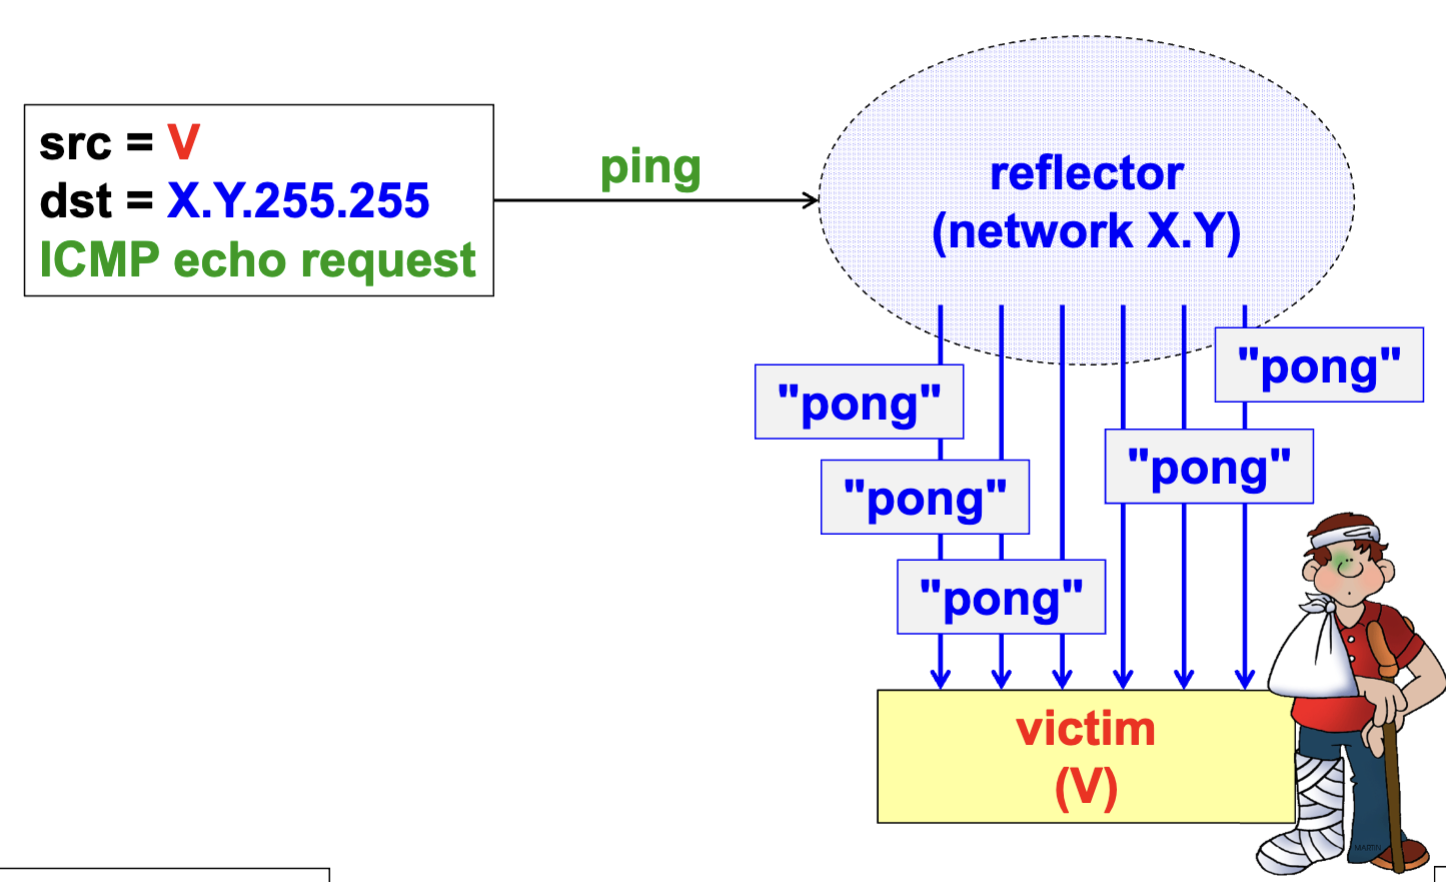
\includegraphics[width=0.5\linewidth]{Images/NetSec/smurfing.png}
        \caption{Smurfing Attack example.}
    \end{figure}
\end{multicols}

Here’s how it works:
\begin{enumerate}
\item \textbf{IP Address Spoofing}: The attacker sends ICMP Echo Request (ping) packets with a spoofed source IP address, set to the target’s IP address.
\item \textbf{Broadcasting}: These ICMP packets are sent to a broadcast address within a network, reaching all devices on that network.
\item \textbf{Amplification}: Each device in the network responds to the ICMP request, sending replies to the spoofed IP address, i.e., the victim.
\item \textbf{Overload}: The victim is overwhelmed by numerous ICMP replies, causing instability or making the system unavailable.
\end{enumerate}

\textbf{Countermeasures:}
\begin{itemize}
\item \textbf{For external attacks}: Reject IP broadcast packets at your network border.
\item \textbf{For internal attacks}: Use network management tools to identify and isolate the attacker.
\end{itemize}

\begin{center}
    \section{Fraggle Attack}
\end{center}

\begin{multicols}{2}
    Type of Distributed Denial of Service (DDoS) attack similar to a smurf attack, but it exploits the User Datagram Protocol (UDP) instead of ICMP. It relies on amplifying traffic by using spoofed UDP packets sent to a network’s broadcast address, overwhelming the victim with responses.

\columnbreak

    \begin{figure}[H]
        \centering
        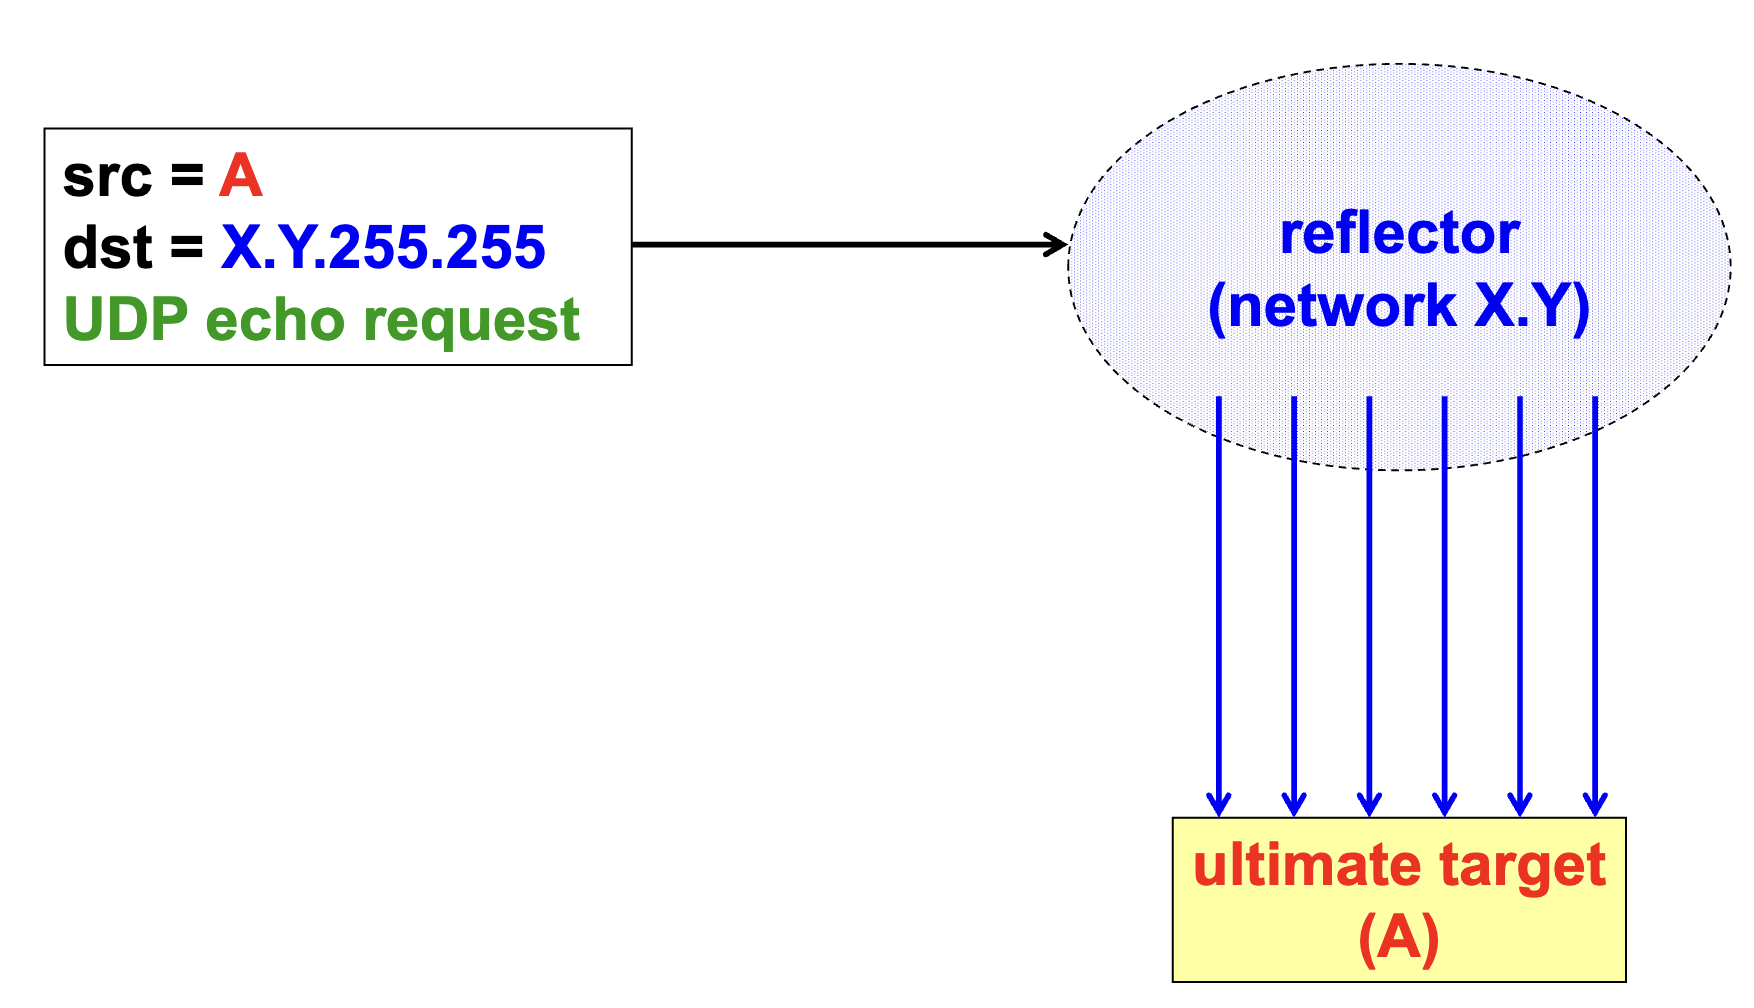
\includegraphics[width=0.5\linewidth]{Images/NetSec/fraggle_attack.png}
        \caption{Fraggle attack example.}
    \end{figure}
\end{multicols}

Here’s how it works:
\begin{enumerate}
\item \textbf{IP Address Spoofing}: The attacker sends UDP packets with a spoofed source IP address, set to the victim’s IP address.
\item \textbf{Broadcasting}: These UDP packets are sent to a broadcast address on a network, targeting specific UDP services.
\item \textbf{Amplification}: All devices in the broadcast network respond to the UDP packets, sending their replies to the victim’s spoofed IP address.
\item \textbf{Overload}: The victim is overwhelmed by the flood of responses, leading to resource exhaustion and potential system unavailability.
\end{enumerate}

\textbf{Countermeasures:}
\begin{itemize}
\item \textbf{Disable IP broadcasting}: Prevent devices in your network from responding to broadcast requests.
\item \textbf{Filter UDP traffic}: Use firewalls to block unnecessary UDP traffic, particularly on ports vulnerable to fraggle attacks (e.g., ports 7 and 19).
\item \textbf{Ingress and egress filtering}: Ensure your network drops packets with spoofed IP addresses to limit the attack’s reach.
\item \textbf{Monitor traffic anomalies}: Use intrusion detection systems (IDS) or other monitoring tools to detect and mitigate unusual UDP traffic patterns.
\end{itemize}

\begin{center}
    \section{ARP Poisoning}
    (Address Resolution Protocol (RFC-826) Poisoning)
\end{center}

ARP is used to discover the Layer 2 (L2) address (MAC address) of a node when its Layer 3 (L3) address (IP address) is known. The result of this resolution is stored in the ARP table of network devices.

Here's how it works:
\begin{enumerate}
    \item \textbf{Unsolicited ARP Replies}: Nodes accept ARP replies even if no ARP request was made.
    \item \textbf{Overwriting Static ARP Entries}: Nodes may overwrite static ARP entries with dynamic entries obtained from an ARP reply.
    \item \textbf{Inconsistent ARP Fields}: The "ar\$sha" ARP field (sender hardware address) in the ARP reply may differ from the source address in the Ethernet frame (802.3 packet).
    \item \textbf{Exploitation by Attack Tools}: Attack tools like Ettercap can be used to carry out ARP poisoning attacks, allowing an attacker to intercept or manipulate network traffic.
\end{enumerate}

Countermeasures:
\begin{enumerate}
    \item \textbf{Static ARP Entries}: Configure static ARP entries on critical network devices to prevent modification by malicious ARP replies.
    \item \textbf{ARP Inspection}: Use Dynamic ARP Inspection (DAI) on managed switches to validate ARP packets.
    \item \textbf{ARP Spoofing Detection Tools}: Use network monitoring tools to detect abnormal ARP behavior and suspicious activity.
\end{enumerate}


\begin{center}
    \section{TCP SYN Flooding}
    (Transmission Control Protocol SYN Flooding)
\end{center}


\begin{multicols}{2}
    Type of Denial of Service (DoS) attack that targets the TCP handshake mechanism. It exploits the way TCP connections are established, overwhelming a server or network device by sending numerous SYN requests without completing the handshake.

\columnbreak

    \begin{figure}[H]
        \centering
        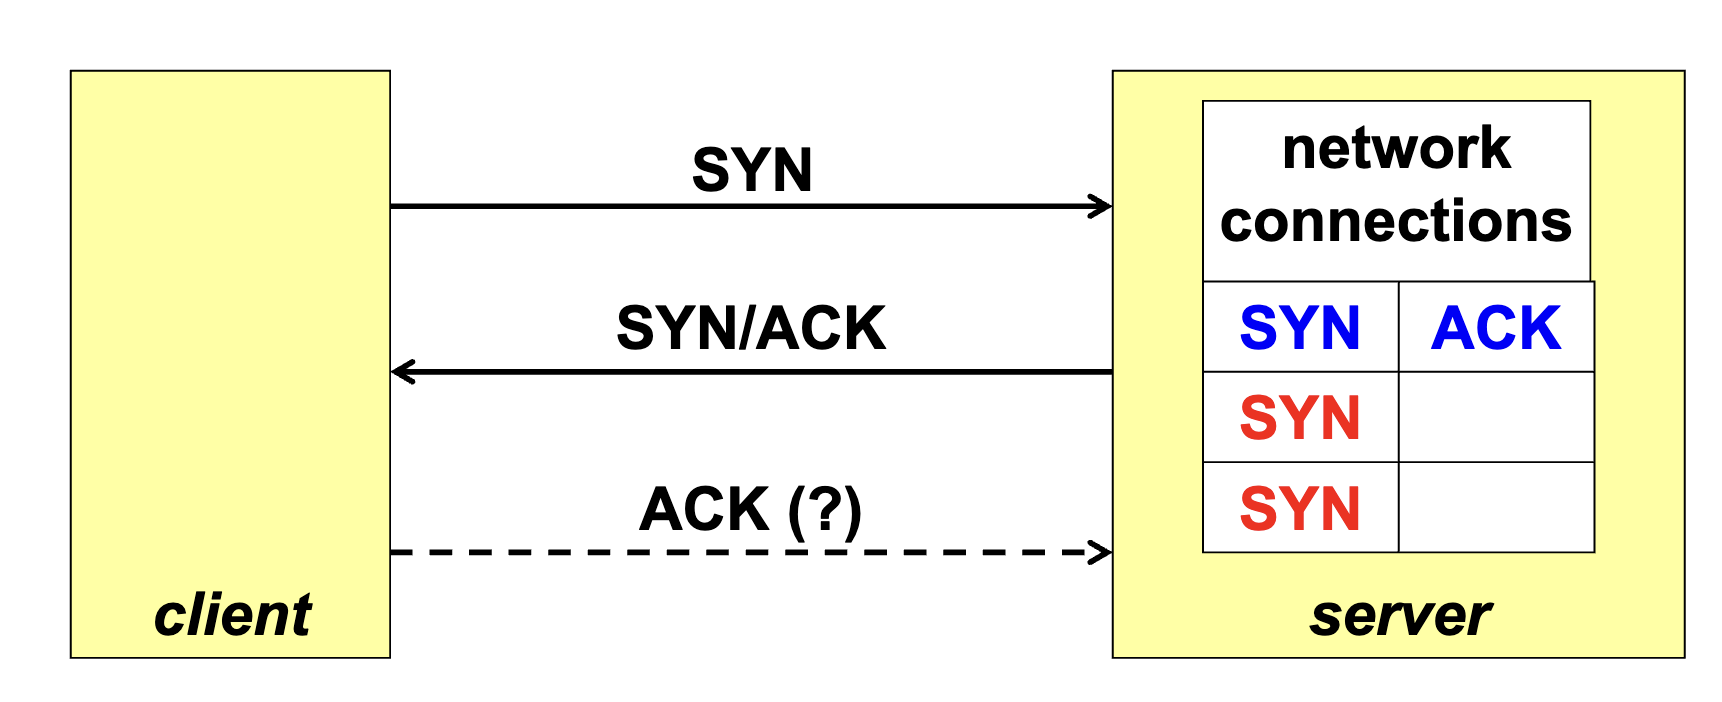
\includegraphics[width=\linewidth]{Images/NetSec/syn_flooding.png}
        \caption{TCP SYN flooding attack example.}
    \end{figure}
\end{multicols}

Here's how it works:
\begin{enumerate}
    \item \textbf{SYN Request}: The attacker sends many TCP packets with the SYN flag set, initiating the three-way handshake but never completing it (i.e., no ACK is sent).
    \item \textbf{Half-Open Connections}: The target system allocates resources (e.g., memory) for each incoming connection in the TCB (Transmission Control Block), waiting for the final ACK to complete the handshake. These connections remain “half-open” and consume system resources.
    \item \textbf{Resource Exhaustion}: The victim’s server or network device becomes overwhelmed by the large number of half-open connections, causing resource exhaustion and potentially making the system unavailable to legitimate users.
\end{enumerate}

Countermeasures:
\begin{enumerate}
    \item \textbf{SYN Cookies}: Eliminate the need for the server to allocate memory resources for half-open connections. When the server receives a SYN packet, it generates a SYN cookie, which is a specially crafted sequence number embedded in the SYN-ACK packet.
    \begin{itemize}
        \item The only approach that is truly effective in completely avoiding the SYN flooding attack.
        \item No resource allocation when receiving a SYN.
        \item The sequence number is computed as a keyed digest.
        \[
            \text{cookie} = \text{HMAC-SHA-256}(K, \text{src} || \text{port})
        \]
        \item The server sends the cookie to the client and waits for the value \(\text{cookie}+1\).
    \end{itemize}
    \item \textbf{Router as "SYN Interceptor"}: Handles the initial stages of the TCP handshake on behalf of the server, reducing the load and risk to the server during a SYN flood attack. Typically, it uses a very short timeout to quickly determine whether the client completes the handshake or not (aggressive timeout).
    \item \textbf{Timeout Reduction}: Reduce the timeout period for half-open connections, limiting how long the server waits for an ACK.
    \item \textbf{Router as "SYN Monitor"}: When the router detects a pending or half-open TCP connection request that has not been completed (i.e., the server hasn’t sent the final ACK), it sends an RST (Reset) packet to terminate the connection.
\end{enumerate}

\begin{multicols}{2}
    \begin{figure}[H]
        \centering
        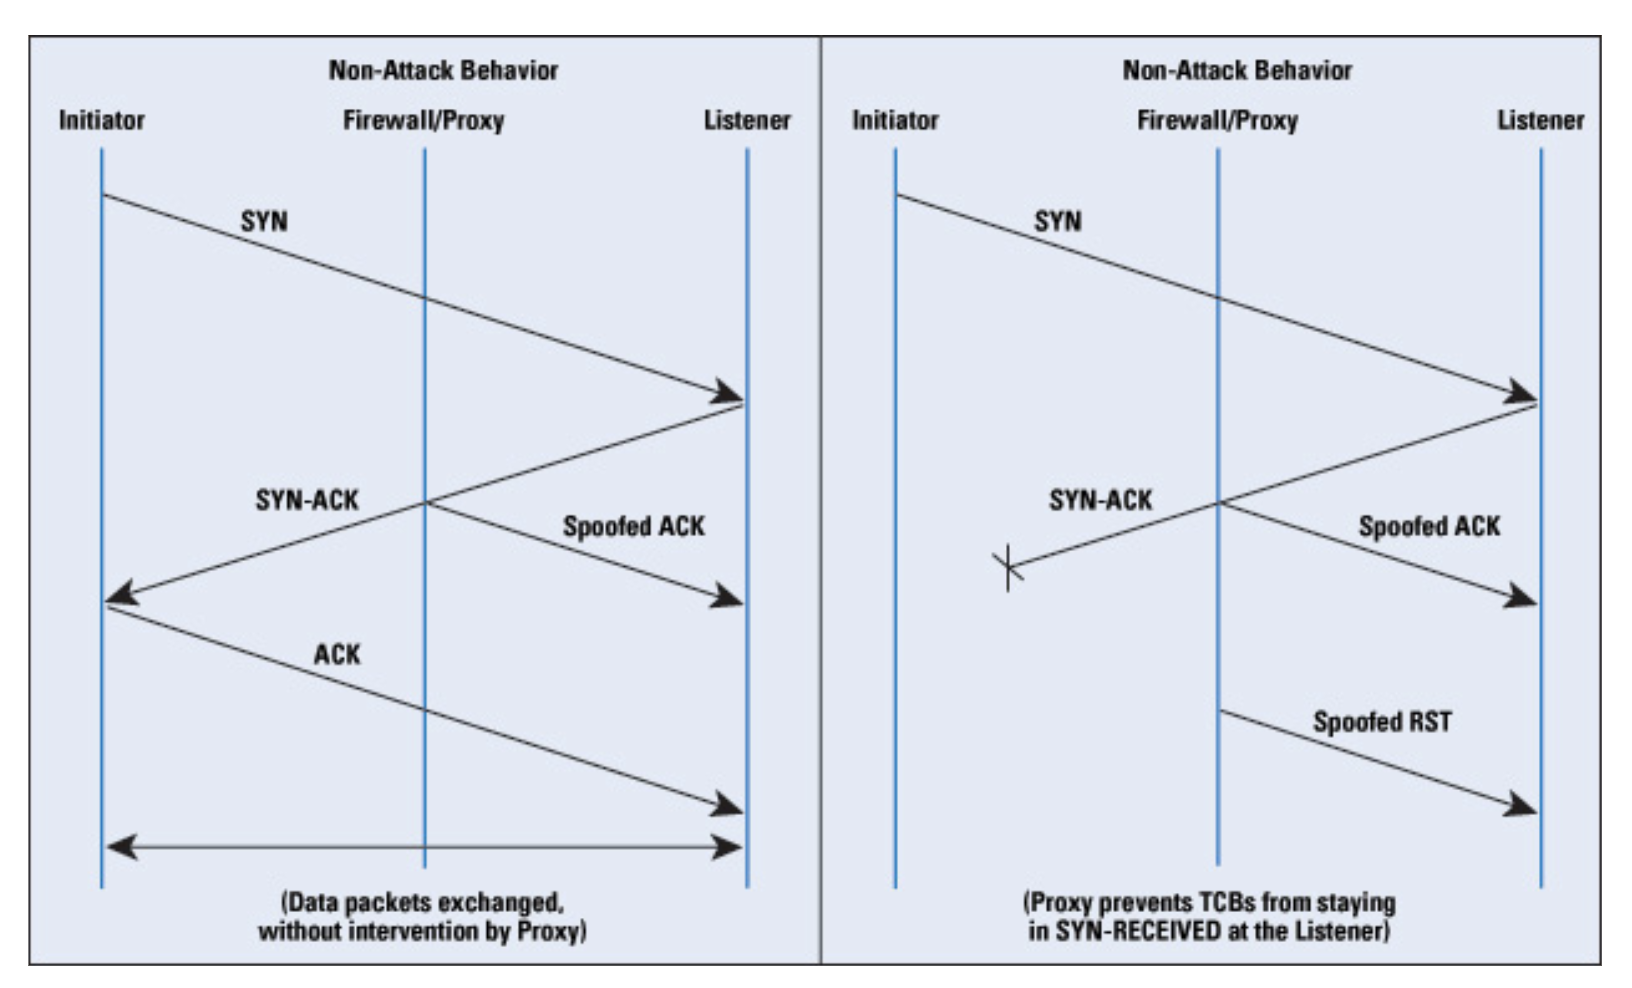
\includegraphics[width=\linewidth]{Images/NetSec/syn_monitor.png}
        \caption{SYN monitor.}
    \end{figure}

\columnbreak

    \begin{figure}[H]
        \centering
        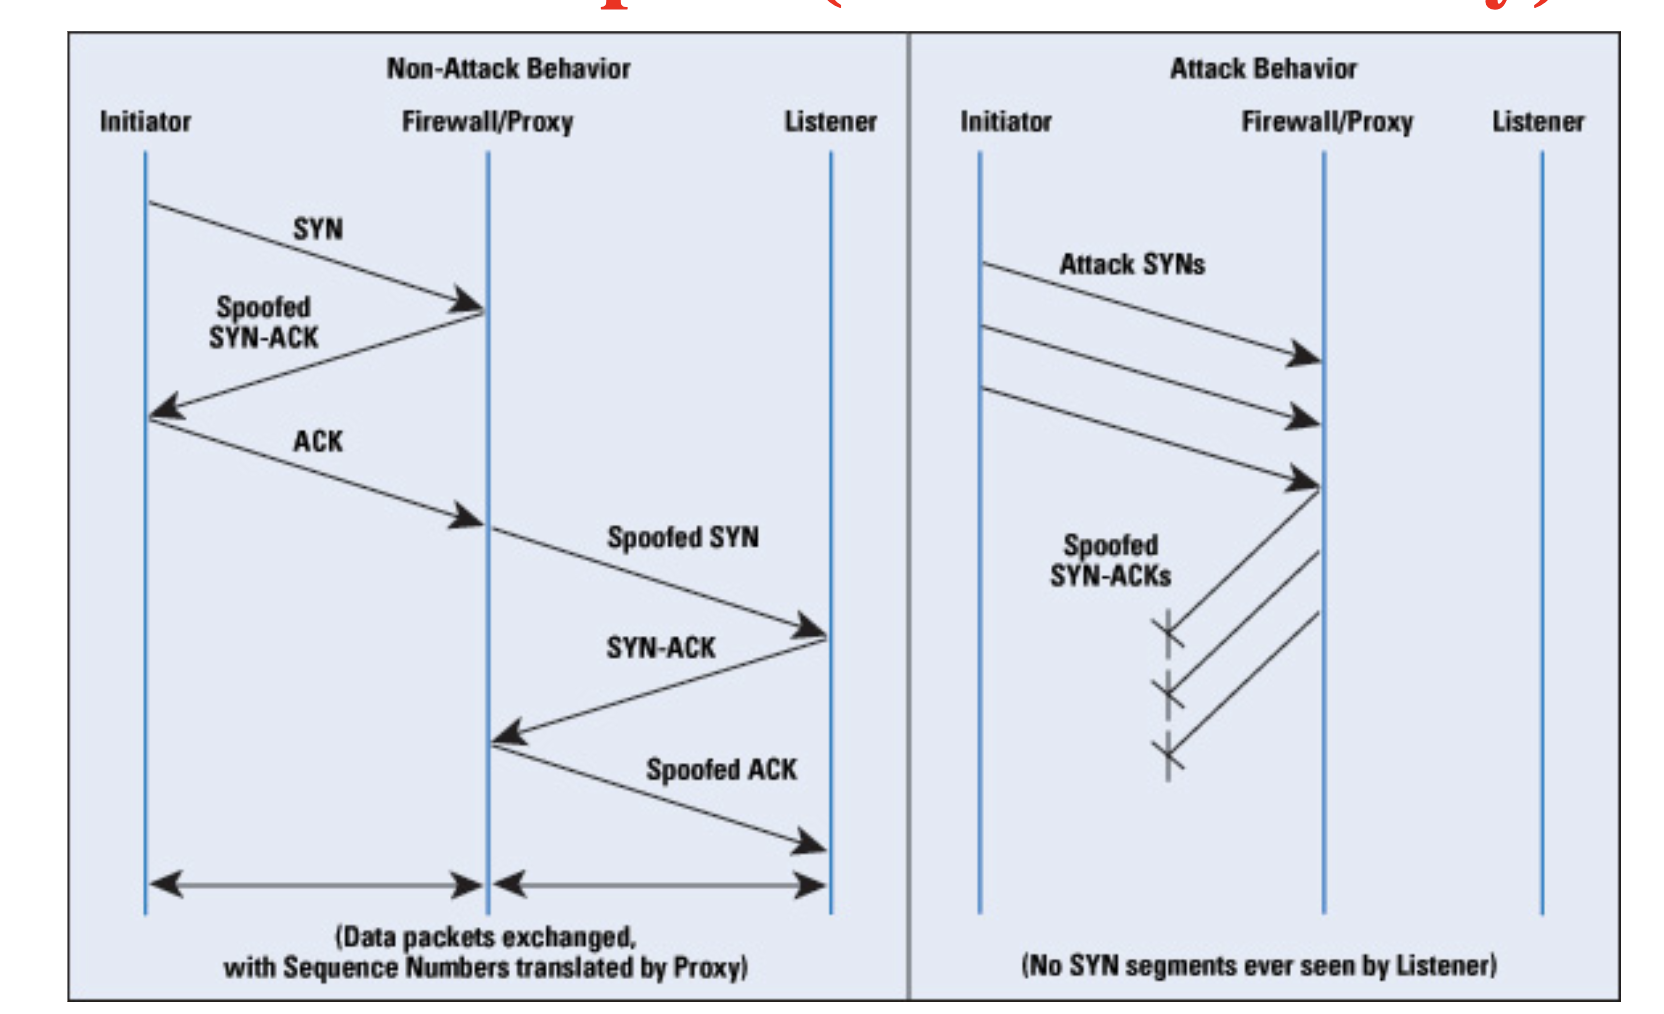
\includegraphics[width=\linewidth]{Images/NetSec/syn_interceptor.png}
        \caption{SYN interceptor.}
    \end{figure}
\end{multicols}

\begin{center}
    \section{DNS}
    (Domain Name System - Security at Level 3)
\end{center}

Here are some types of attacks listed:
\begin{itemize}
    \item DNS \textbf{Cache Poisoning v1} - \textcolor{Blue}{Request-based}, fig:\ref{fig:dns_pv1}: 
    The user attempts to resolve a query by addressing a malicious nameserver. An attacker, then, injects false DNS records (even for non-requested domains) into the cache of a DNS resolver (overwriting existing ones), redirecting traffic to malicious sites or disrupting services. This attack exploits vulnerabilities in how DNS servers handle responses without proper validation.
    \item DNS \textbf{Cache Poisoning v2}, fig:\ref{fig:dns_pv2}: 
    A more advanced form of cache poisoning exploits weaknesses in DNS security. The attacker sends a query to a DNS resolver and simultaneously provides a forged (incorrect) answer. This fake response includes malicious DNS records, designed to be accepted and cached by the victim’s resolver. As a result, the attacker can redirect traffic or disrupt services.
    \begin{itemize}
        \item The fake nameserver must respond faster than the authoritative nameservers for the queried domain, which typically include at least three servers (with one being off-site).
    \end{itemize}
    \item DNS \textbf{Flash Crowd}: sudden and massive surge of DNS queries to specific domain names, often caused by an unexpected event, like viral content, breaking news, or a popular service announcement. This can result in a strain on DNS servers, potentially leading to delays or service degradation.
\end{itemize}

\begin{multicols}{2}
    \begin{figure}[H]
        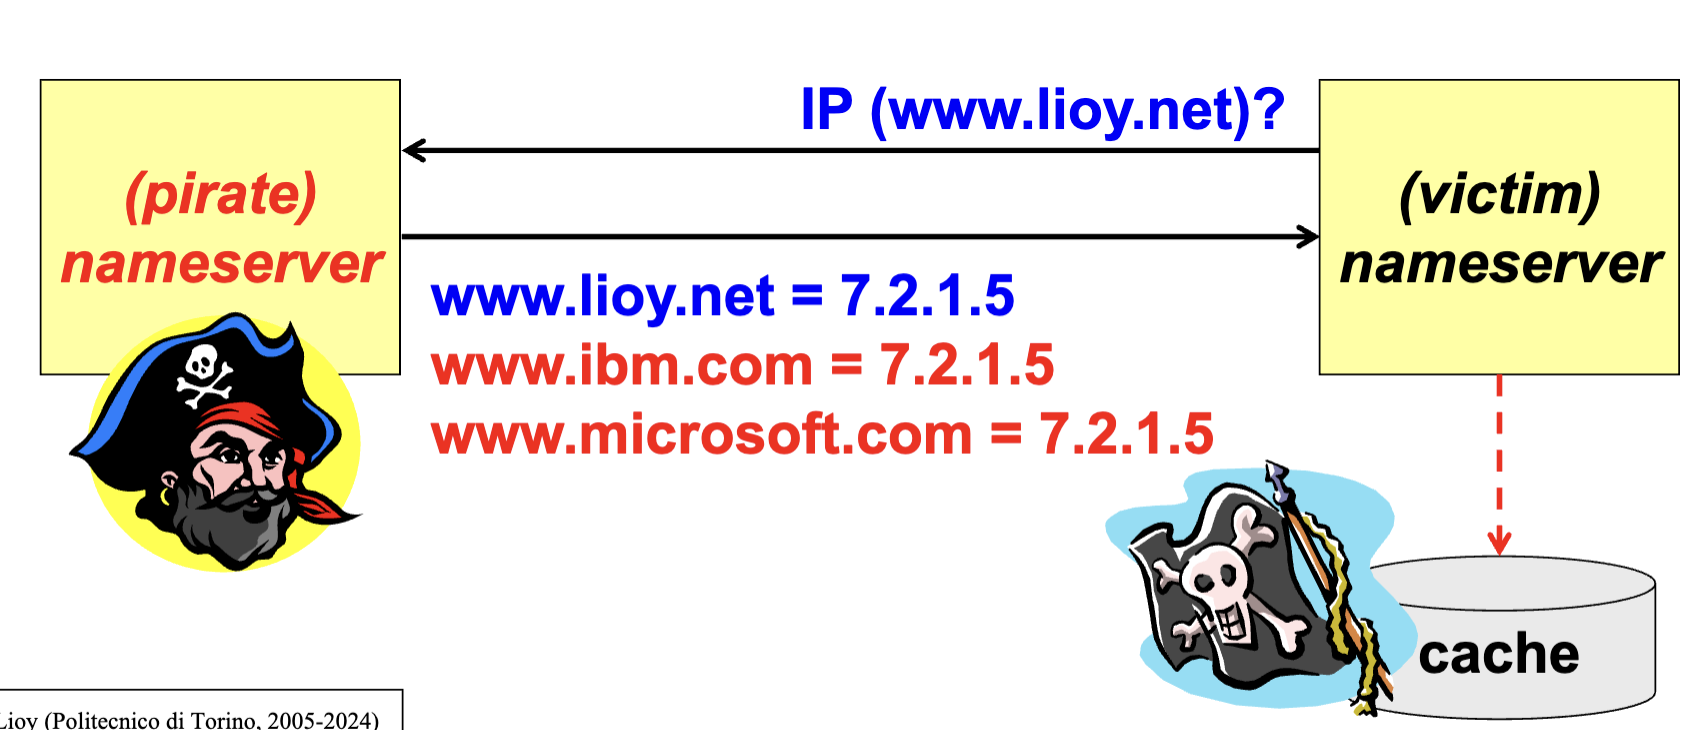
\includegraphics[width=\linewidth]{Images/NetSec/dns_cache_pv1.png}
        \caption{DNS cache poisoning v1.}
        \label{fig:dns_pv1}
      \end{figure}

\columnbreak

  
  \begin{figure}[H]
      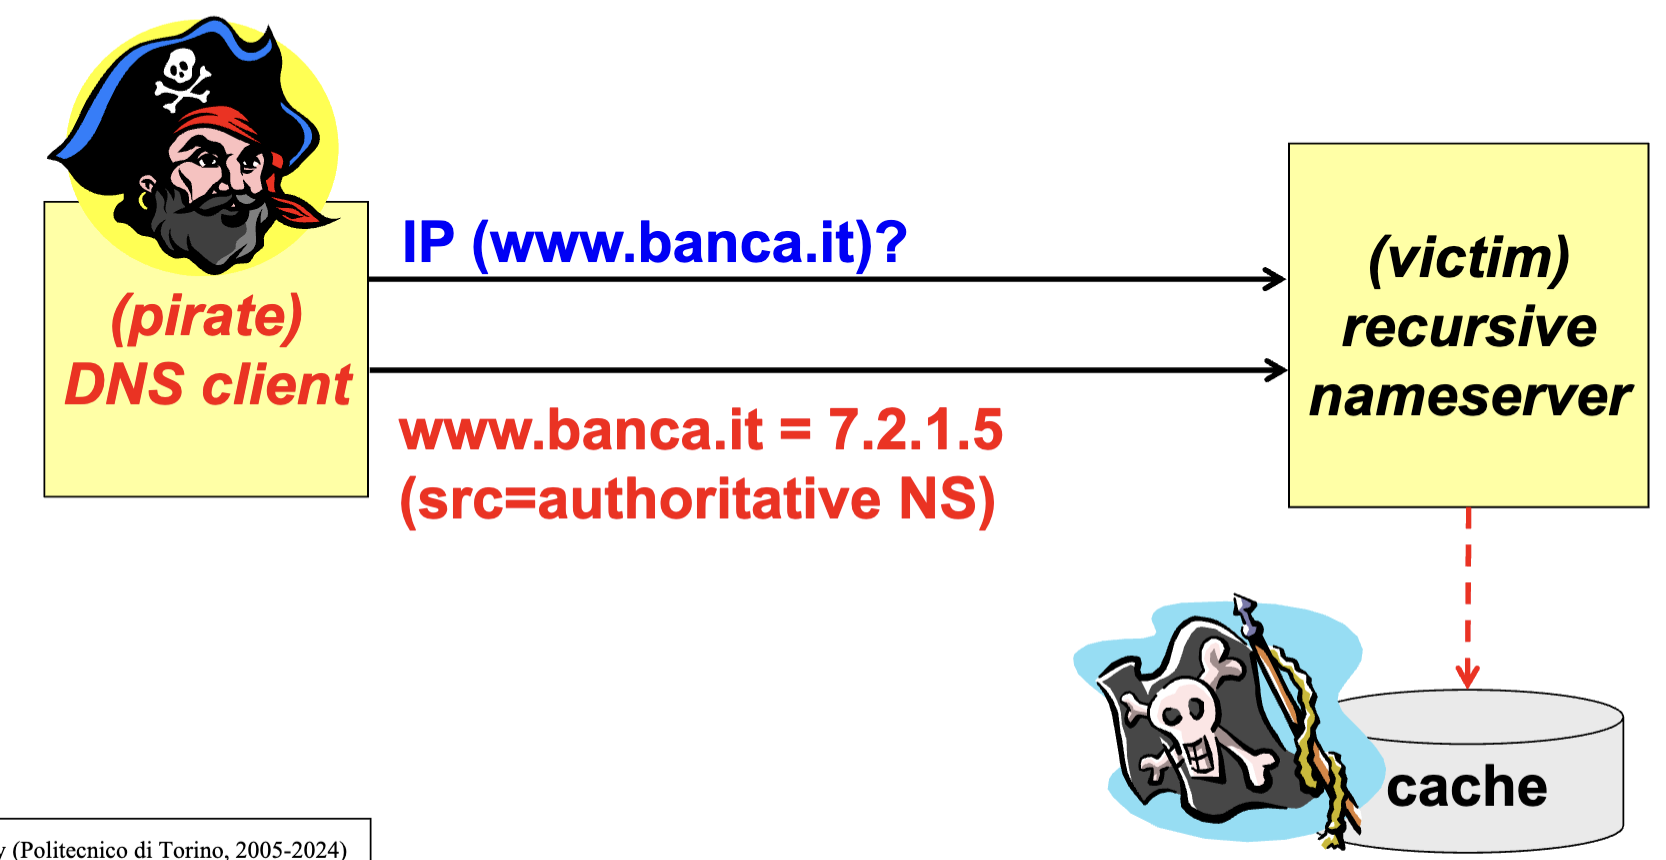
\includegraphics[width=\linewidth]{Images/NetSec/dns_cache_pv2.png}
      \caption{DNS cache poisoning v2.}
      \label{fig:dns_pv2}
    \end{figure}
    
\end{multicols}


\begin{center}
    \section{Hiccup}
    (The term isn’t officially standardized)
\end{center}
A \textbf{Denial of Service (DoS) attack} that exploits periodic unavailability or instability in a system’s performance. This type of attack involves causing brief disruptions or intermittent delays in service rather than sustaining a continuous outage.

Key features:
\begin{itemize}
    \item \textbf{Intermittent Disruption:} Instead of overwhelming the target continuously, the attacker sends \underline{bursts} of malicious traffic or \underline{sporadically} exploits vulnerabilities, making the attack more difficult to detect.
    \item \textbf{Impact:} The attack degrades user experience (e.g., introducing lag or delays in applications), rendering the service unreliable without fully taking it offline.
    \item \textbf{Targets:} Common targets include DNS servers, application servers, or APIs with specific vulnerabilities or low tolerance to periodic spikes.
\end{itemize}

% --------











\section{Attack Vectors}

\begin{table}[H]
    \centering
    \begin{tabular}{|p{3cm}|p{12cm}|}\hline
    \rowcolor{blue!10}
    \textbf{Vector} 
        & \textbf{Description}  
    \\ \hline

    Trojan
        & Appears as legitimate software or a harmless file to deceive users into installing it. Contains a dangerous payload and is often used to create a Man At The End or a Man In The Browser.
    \\ \hline
    
    Virus
        & Attaches itself to legitimate files or programs and spreads by infecting other files on a system. Is propagated by humans (often involuntarily).
    \\ \hline

    Worm
        & Self-replicating malware that spreads across networks without requiring user intervention. Unlike a virus, a worm does not need to attach itself to a file or program.
    \\ \hline

    Backdoor
        & Unauthorized access point, it allow